\documentclass[11pt,letterpaper,onecolumn,notitlepage]{article}
\usepackage[english]{babel}
\usepackage[compact]{titlesec}
\usepackage[titles]{tocloft}
\usepackage{%
  float,
  amssymb,
  amsmath,
  graphicx,
  fullpage,
  textcomp,
  gensymb,
  hyperref,
  listings,
  caption,
  sectsty,
  bm,
  times,
  parskip
}
\usepackage[framed,numbered,autolinebreaks,useliterate]{../sty/mcode}

\lstset{breakatwhitespace=false}

\newcommand{\figurepath}{../fig/hw2}
\newcommand{\codepath}{../include/code/hw2}

\sectionfont{\fontsize{16pt}{16pt}\selectfont\bfseries\sffamily}
\subsectionfont{\fontsize{13pt}{13pt}\selectfont\sffamily}
\subsubsectionfont{\fontsize{12pt}{12pt}\selectfont\sffamily}
\paragraphfont{\fontsize{11pt}{11pt}\selectfont\bfseries}

\makeatletter
\renewcommand\section{\@startsection{section}{1}{\z@}%
{-3.5ex\@plus-1ex\@minus-0.2ex}%
{1.0ex\@plus0.2ex}%
{\fontsize{12pt}{12pt}\selectfont\bfseries\sffamily}}
\makeatother

\makeatletter
\renewcommand\subsection{\@startsection{subsection}{1}{\z@}%
{-3.5ex\@plus-1ex\@minus-0.2ex}%
{0.5ex\@plus0.2ex}%
{\fontsize{10pt}{10pt}\selectfont\bfseries\sffamily}}
\makeatother

%------------------------------------------------------------------------
\setlength\cftparskip{-3pt}
\setlength\cftbeforesecskip{1pt}
\setlength\cftaftertoctitleskip{1pt}
\cftsetindents{figure}{0em}{1.5em}
\makeatletter
\renewcommand{\@dotsep}{4.5}
\renewcommand{\cftdotsep}{4.5}
\renewcommand{\cftsecdotsep}{4.5}
\renewcommand{\@tocrmarg}{4.55em}
\makeatother
\renewcommand\cftsecfont{\normalfont}
\renewcommand\cftsecpagefont{\normalfont}
\renewcommand{\cftsecleader}{\cftdotfill{\cftsecdotsep}}
%------------------------------------------------------------------------

\titleformat{\chapter}[display]{\huge\bf}{Lecture \thechapter}{0pt}{\Large}

\title{\textbf{Title}}
\author{Daniel Wiese \\ Department of Mechanical Engineering \\ Massachusetts Institute of Technology}
\date{\today}

\begin{document}

\begin{titlepage}
  \begin{center}
    \rule{\linewidth}{0.01in} \\[0.25in]
    {\huge\bfseries 16.323 Optimal Control}\\[0.4cm]
    \rule{\linewidth}{0.01in} \\[0.25in]

    \textsc{\LARGE Problem Set 2}\\[0.15in]
    \large Due: Thursday, March 6, 2014 \\[1.0in]
    
\includegraphics[width=1.5in]{../fig/mit-seal.pdf}\\[3.0in]

    % Author and instructor
    \begin{minipage}{0.4\textwidth}
      \begin{flushleft} \large
        \emph{Author:}\\
        Daniel \textsc{Wiese}
        \vfill
      \end{flushleft}
    \end{minipage}
    \begin{minipage}{0.4\textwidth}
      \begin{flushright} \large
        \emph{Instructor:} \\
        Prof.~Steven \textsc{Hall} \\
      \end{flushright}
    \end{minipage} \\
    \vfill
  \end{center}
\end{titlepage}

\clearpage
\section*{(1) Automatic Differentiation}

The problem is to find the optimal controller for the inverted pendulum, with dynamics given by

\begin{equation*}
  \ddot{\theta}(t)=\sin(\theta(t))+u
\end{equation*}

$\theta=0$ corresponds to vertical.
The cost functional to minimize is

\begin{equation*}
  J=\int_{0}^{t_{f}}(\theta^{2}+\rho u^{2})dt
\end{equation*}

For the purposes of this problem, we will take $t_{f}=10$, $\rho=10$.

\subsection*{1. Adjoint Method}

% Automatic differentiation (AD), also called algorithmic differentiation or computational differentiation,[1][2] is a set of techniques to numerically evaluate the derivative of a function specified by a computer program.
% AD exploits the fact that every computer program, no matter how complicated, executes a sequence of elementary arithmetic operations (addition, subtraction, multiplication, division, etc.) and elementary functions (exp, log, sin, cos, etc.).
% By applying the chain rule repeatedly to these operations, derivatives of arbitrary order can be computed automatically

The code was provided that integrates the given state equation using a second order Runge-Kutta solver.
This function took as an input a control vector $u$ over the specified simulation time, and integrated the equations of motion using this control input.
The cost was evaluated and outputted from the function, as was the state trajectory $x$.
The reverse accumulation adjoint method was used to write the function \texttt{pendulum\textunderscore{}b.m} which contains both the forward code described above and the reverse code.
The reverse code used automatic differentiation to return the derivative of the cost function with respect to the input $u$, in addition to the other outputs already described.
The code can be found in the appendix.

\subsection*{2. Finding Optimal Control History}

Using the function \texttt{pendulum\textunderscore{}b.m} above, the gradient, which was obtained using automatic differentiation, can be passed to \texttt{fminunc.m} to determine the optimal control history $u^{*}$.
This control history was then given to the pendulum to bring the pendulum to the upright position.
Plots of the optimal control history and state history are shown below.

\begin{figure}[H]
  \centering
  \begin{minipage}{.48\textwidth}
    \centering
    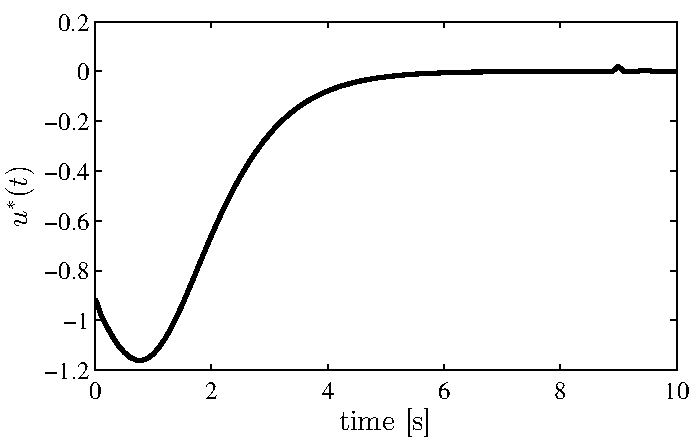
\includegraphics[width=3in]{\figurepath/prob1_control.pdf}
    \caption{Optimal control input $u^{*}(t)$\label{fig:part1_control}}
  \end{minipage}
  \hfill
  \begin{minipage}{.48\textwidth}
    \centering
    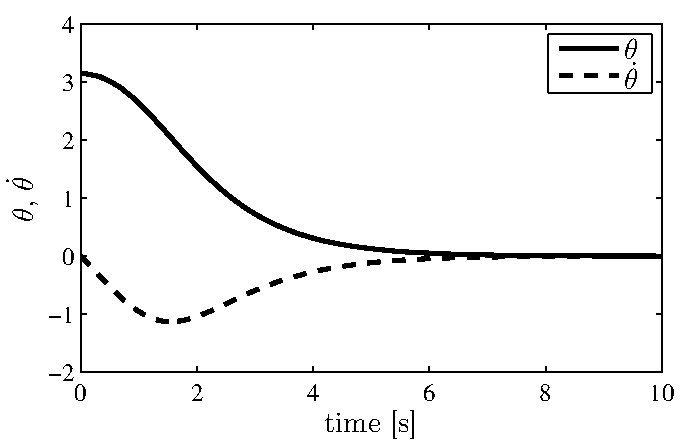
\includegraphics[width=3in]{\figurepath/prob1_state.pdf}
    \caption{State history with optimal control input\label{fig:part1_state}}
  \end{minipage}
\end{figure}

\clearpage
\section*{(2) Discrete Time LQ-Tracking Problem}

The discrete-time linear quadratic tracking problem is to minimize the cost

\begin{equation*}
  J=\sum_{k=0}^{N}\underbrace{\frac{1}{2}\left[(r_{k}-C_{k}x_{k})^{\top}(r_{k}-C_{k}x_{k})+u_{k}^{\top}R_{k}u_{k}\right]}_{g_{k}(x_{k},u_{k})}
\end{equation*}

subject to the constraint that the dynamics are

\begin{equation*}
  x_{k+1}=A_{k}x_{k}+B_{k}u_{k}
\end{equation*}

The goal is for the performance variables $z_{k}=C_{k}x_{k}$ to track the reference input $r_{k}$ as closely as possible, using minimum control effort.

\subsection*{1. Use dynamic programming to find the control that minimizes the cost.}

Define the terminal cost as

\begin{equation*}
  V_{N}(x_{N})=\min_{u_{N}}g_{N}(x_{N},u_{N})
\end{equation*}

which is the cost associated with the the final state of the system.
From the dynamics we can see that a control input $u_{N}$ has no influence on the state $x_{N}$, and thus no influence on the terminal cost through the dynamics.
Because of this, the optimal control $u_{N}=0$, and the terminal cost can be written as

\begin{equation*}
  V_{N}(x_{N})=\frac{1}{2}\left[(r_{N}-C_{N}x_{N})^{\top}(r_{N}-C_{N}x_{N})\right]
\end{equation*}

The cost to go at $N-1$ is the cost associated with going from $N-1$ to $N$, as well as the cost associated with state $N$.
This can be written as

\begin{equation*}
  V_{N-1}(x_{N-1})=\min_{u_{N-1}}\left\{g_{N-1}(x_{N-1},u_{N-1})+V_{N}(x_{N})\right\}
\end{equation*}

Inserting the expression for $g_{N-1}$ and $V_{N}$ this becomes

\begin{equation*}
  \begin{split}
    V_{N-1}(x_{N-1})=\min_{u_{N-1}}&\biggr\{\frac{1}{2}\left[(r_{N-1}-C_{N-1}x_{N-1})^{\top}(r_{N-1}-C_{N-1}x_{N-1})+u_{N-1}^{\top}R_{N-1}u_{N-1}\right] \\
    &+\frac{1}{2}\left[(r_{N}-C_{N}x_{N})^{\top}(r_{N}-C_{N}x_{N})\right]\biggr\}
  \end{split}
\end{equation*}

Using the plant dynamics $x_{N}=A_{N-1}x_{N-1}+B_{N-1}u_{N-1}$ and simplifying the subscript notation, this becomes

\begin{equation*}
  \begin{split}
    V_{N-1}(x_{N-1})=\min_{u_{N-1}}&\biggr\{\frac{1}{2}\left[(r-Cx)^{\top}(r-Cx)+u^{\top}Ru\right]_{N-1} \\
    &+\frac{1}{2}\left[\bigr(r_{N}-C_{N}(A_{N-1}x_{N-1}+B_{N-1}u_{N-1})\bigr)^{\top}\bigr(r_{N}-C_{N}(A_{N-1}x_{N-1}+B_{N-1}u_{N-1})\bigr)\right]\biggr\}
  \end{split}
\end{equation*}

Simplifying

\begin{equation*}
  \begin{split}
    V_{N-1}(x_{N-1})=\min_{u_{N-1}}&\biggr\{\frac{1}{2}\left[r^{\top}r-x^{\top}C^{\top}r-r^{\top}Cx+x^{\top}C^{\top}Cx+u^{\top}Ru\right]_{N-1} \\
    &+\frac{1}{2}\left[\bigr(r_{N}^{\top}-(Ax+Bu)_{N-1}^{\top}C_{N}^{\top}\bigr)\bigr(r_{N}-C_{N}(Ax+Bu)_{N-1}\bigr)\right]\biggr\}
  \end{split}
\end{equation*}

Simplifying

\begin{equation*}
  \begin{split}
    V_{N-1}&(x_{N-1})=\min_{u_{N-1}}\biggr\{\frac{1}{2}\left[r^{\top}r-2r^{\top}Cx+x^{\top}C^{\top}Cx+u^{\top}Ru\right]_{N-1} \\
    &+\frac{1}{2}\left[r_{N}^{\top}r_{N}-(Ax+Bu)_{N-1}^{\top}C_{N}^{\top}r_{N}-r_{N}^{\top}C_{N}(Ax+Bu)_{N-1}+(Ax+Bu)_{N-1}^{\top}C_{N}^{\top}C_{N}(Ax+Bu)_{N-1}\right]\biggr\}
  \end{split}
\end{equation*}

Simplifying

\begin{equation*}
  \begin{split}
    V_{N-1}&(x_{N-1})=\min_{u_{N-1}}\biggr\{\frac{1}{2}\left[r^{\top}r-2r^{\top}Cx+x^{\top}C^{\top}Cx+u^{\top}Ru\right]_{N-1} \\
    &+\frac{1}{2}\bigr[r_{N}^{\top}r_{N}-2(Ax+Bu)_{N-1}^{\top}C_{N}^{\top}r_{N} \\
    &+x_{N-1}^{\top}A_{N-1}C_{N}^{\top}C_{N}A_{N-1}x_{N-1}
    +u_{N-1}^{\top}B_{N-1}^{\top}C_{N}^{\top}C_{N}A_{N-1}x_{N-1} \\
    &+x_{N-1}^{\top}A_{N-1}C_{N}^{\top}C_{N}B_{N-1}u_{N-1}
    +u_{N-1}^{\top}B_{N-1}^{\top}C_{N}^{\top}C_{N}B_{N-1}u_{N-1}
    \bigr]\biggr\}
  \end{split}
\end{equation*}

Simplifying

\begin{equation*}
  \begin{split}
    V_{N-1}&(x_{N-1})=\min_{u_{N-1}}\biggr\{\frac{1}{2}\left[r^{\top}r-2r^{\top}Cx+x^{\top}C^{\top}Cx+u^{\top}Ru\right]_{N-1} \\
    &+\frac{1}{2}\bigr[r_{N}^{\top}r_{N}
    -2x_{N-1}^{\top}A_{N-1}^{\top}C_{N}^{\top}r_{N}-2u_{N-1}^{\top}B_{N-1}^{\top}C_{N}^{\top}r_{N} \\
    &+x_{N-1}^{\top}A_{N-1}C_{N}^{\top}C_{N}A_{N-1}x_{N-1}
    +2u_{N-1}^{\top}B_{N-1}^{\top}C_{N}^{\top}C_{N}A_{N-1}x_{N-1} \\
    &+u_{N-1}^{\top}B_{N-1}^{\top}C_{N}^{\top}C_{N}B_{N-1}u_{N-1}
    \bigr]\biggr\}
  \end{split}
\end{equation*}

And to minimize we evaluate $\frac{\partial}{\partial u_{N-1}}V_{N-1}(x_{N-1})$ as follows

\begin{equation*}
  \begin{split}
    \frac{\partial}{\partial u_{N-1}}V_{N-1}(x_{N-1})=\frac{\partial}{\partial u_{N-1}}\frac{1}{2}\biggr\{&u_{N-1}^{\top}R_{N-1}u_{N-1}-2u_{N-1}^{\top}B_{N-1}^{\top}C_{N}^{\top}r_{N} \\
    &+2u_{N-1}^{\top}B_{N-1}^{\top}C_{N}^{\top}C_{N}A_{N-1}x_{N-1}+
    u_{N-1}^{\top}B_{N-1}^{\top}C_{N}^{\top}C_{N}B_{N-1}u_{N-1}\biggr\}
  \end{split}
\end{equation*}

Evaluating the derivative

\begin{equation*}
  \begin{split}
    \frac{\partial}{\partial u_{N-1}}V_{N-1}(x_{N-1})=\biggr\{R_{N-1}u_{N-1}-B_{N-1}^{\top}C_{N}^{\top}r_{N}+B_{N-1}^{\top}C_{N}^{\top}C_{N}A_{N-1}x_{N-1}+B_{N-1}^{\top}C_{N}^{\top}C_{N}B_{N-1}u_{N-1}\biggr\}
  \end{split}
\end{equation*}

Simplifying

\begin{equation*}
  \begin{split}
    \frac{\partial}{\partial u_{N-1}}V_{N-1}(x_{N-1})=(R_{N-1}+B_{N-1}^{\top}C_{N}^{\top}C_{N}B_{N-1})u_{N-1}-(B_{N-1}^{\top}C_{N}^{\top}r_{N}-B_{N-1}^{\top}C_{N}^{\top}C_{N}A_{N-1}x_{N-1})
  \end{split}
\end{equation*}

And the optimal control input $u_{N-1}^{*}$ is the control such that $\frac{\partial V_{N-1}}{\partial u_{N-1}}=$, with the second derivative positive.
This gives

\begin{equation*}
  \boxed{%
    u_{N-1}^{*}=(R_{N-1}+B_{N-1}^{\top}C_{N}^{\top}C_{N}B_{N-1})^{-1}(B_{N-1}^{\top}C_{N}^{\top}r_{N}-B_{N-1}^{\top}C_{N}^{\top}C_{N}A_{N-1}x_{N-1})
  }
\end{equation*}

Which can be written as

\begin{equation*}
  \addtolength{\fboxsep}{5pt}
  \boxed{%
    \begin{split}
      u_{N-1}^{*}&=G_{N}r_{N}-F_{N}x_{N-1} \\
      G_{N}&=(R_{N-1}+B_{N-1}^{\top}C_{N}^{\top}C_{N}B_{N-1})^{-1}B_{N-1}^{\top}C_{N}^{\top} \\
      F_{N}&=(R_{N-1}+B_{N-1}^{\top}C_{N}^{\top}C_{N}B_{N-1})^{-1}B_{N-1}^{\top}C_{N}^{\top}C_{N}A_{N-1}
    \end{split}
  }
\end{equation*}

Plugging this expression for the control law into $V_{N-1}(x_{N-1})$ we have

\begin{equation*}
  \begin{split}
    V_{N-1}&(x_{N-1})=\min_{u_{N-1}}\frac{1}{2}\biggr\{
    \left[r^{\top}r-2r^{\top}Cx+x^{\top}C^{\top}Cx\right]_{N-1}+(G_{N}r_{N}-F_{N}x_{N-1})^{\top}R_{N-1}(G_{N}r_{N}-F_{N}x_{N-1}) \\
    &+r_{N}^{\top}r_{N}
    -2x_{N-1}^{\top}A_{N-1}^{\top}C_{N}^{\top}r_{N}-2(G_{N}r_{N}-F_{N}x_{N-1})^{\top}B_{N-1}^{\top}C_{N}^{\top}r_{N} \\
    &+x_{N-1}^{\top}A_{N-1}C_{N}^{\top}C_{N}A_{N-1}x_{N-1}
    +2(G_{N}r_{N}-F_{N}x_{N-1})^{\top}B_{N-1}^{\top}C_{N}^{\top}C_{N}A_{N-1}x_{N-1} \\
    &+(G_{N}r_{N}-F_{N}x_{N-1})^{\top}B_{N-1}^{\top}C_{N}^{\top}C_{N}B_{N-1}(G_{N}r_{N}-F_{N}x_{N-1})
    \biggr\}
  \end{split}
\end{equation*}

Simplifying

\begin{equation*}
  \begin{split}
    V_{N-1}&(x_{N-1})=\min_{u_{N-1}}\frac{1}{2}\biggr\{
    \left[r^{\top}r-2r^{\top}Cx+x^{\top}C^{\top}Cx\right]_{N-1}
    +(r_{N}^{\top}G_{N}^{\top}-x_{N-1}^{\top}F_{N}^{\top})R_{N-1}(G_{N}r_{N}-F_{N}x_{N-1}) \\
    &+r_{N}^{\top}r_{N}
    -2x_{N-1}^{\top}A_{N-1}^{\top}C_{N}^{\top}r_{N}
    -2(r_{N}^{\top}G_{N}^{\top}-x_{N-1}^{\top}F_{N}^{\top})B_{N-1}^{\top}C_{N}^{\top}r_{N} \\
    &+x_{N-1}^{\top}A_{N-1}C_{N}^{\top}C_{N}A_{N-1}x_{N-1}
    +2(r_{N}^{\top}G_{N}^{\top}-x_{N-1}^{\top}F_{N}^{\top})B_{N-1}^{\top}C_{N}^{\top}C_{N}A_{N-1}x_{N-1} \\
    &+(r_{N}^{\top}G_{N}^{\top}-x_{N-1}^{\top}F_{N}^{\top})B_{N-1}^{\top}C_{N}^{\top}C_{N}B_{N-1}(G_{N}r_{N}-F_{N}x_{N-1})
    \biggr\}
  \end{split}
\end{equation*}

Simplifying

\begin{equation*}
  \begin{split}
    V_{N-1}&(x_{N-1})=\min_{u_{N-1}}\frac{1}{2}\biggr\{
    \left[r^{\top}r-2r^{\top}Cx+x^{\top}C^{\top}Cx\right]_{N-1}
    +r_{N}^{\top}G_{N}^{\top}R_{N-1}G_{N}r_{N}
    +x_{N-1}^{\top}F_{N}^{\top}R_{N-1}F_{N}x_{N-1} \\
    &-2r_{N}^{\top}G_{N}^{\top}R_{N-1}F_{N}x_{N-1} \\
    &+r_{N}^{\top}r_{N}
    -2r_{N}^{\top}C_{N}A_{N-1}x_{N-1}
    -2r_{N}^{\top}G_{N}^{\top}B_{N-1}^{\top}C_{N}^{\top}r_{N}
    +2x_{N-1}^{\top}F_{N}^{\top}B_{N-1}^{\top}C_{N}^{\top}r_{N} \\
    &+x_{N-1}^{\top}A_{N-1}C_{N}^{\top}C_{N}A_{N-1}x_{N-1}
    +2r_{N}^{\top}G_{N}^{\top}B_{N-1}^{\top}C_{N}^{\top}C_{N}A_{N-1}x_{N-1} \\
    &-2x_{N-1}^{\top}F_{N}^{\top}B_{N-1}^{\top}C_{N}^{\top}C_{N}A_{N-1}x_{N-1} \\
    &+r_{N}^{\top}G_{N}^{\top}B_{N-1}^{\top}C_{N}^{\top}C_{N}B_{N-1}G_{N}r_{N}
    -2r_{N}^{\top}G_{N}^{\top}B_{N-1}^{\top}C_{N}^{\top}C_{N}B_{N-1}F_{N}x_{N-1} \\
    &+x_{N-1}^{\top}F_{N}^{\top}B_{N-1}^{\top}C_{N}^{\top}C_{N}B_{N-1}F_{N}x_{N-1}
    \biggr\}
  \end{split}
\end{equation*}

This cost-to-go function can be expressed as

\begin{equation*}
  \fontsize{6pt}{1pt}\selectfont
  \addtolength{\fboxsep}{5pt}
  \boxed{%
    \begin{split}
      V_{N-1}(x_{N-1})&=\frac{1}{2}x_{N-1}^{\top}P_{N-1}x_{N-1}+q_{N-1}x_{N-1}+s_{N-1} \\
      P_{N-1}&=\frac{1}{2}\bigr(C_{N-1}^{\top}C_{N-1}+F_{N}^{\top}R_{N-1}F_{N}+A_{N-1}^{\top}C_{N}^{\top}C_{N}A_{N-1}-2F_{N}^{\top}B_{N-1}^{\top}C_{N}^{\top}C_{N}A_{N-1}+F_{N}^{\top}B_{N-1}^{\top}C_{N}^{\top}C_{N}B_{N-1}F_{N}\bigr) \\
      q_{N-1}&=-r_{N-1}^{\top}C_{N-1}-r_{N}^{\top}G_{N}^{\top}R_{N-1}F_{N}-r_{N}^{\top}C_{N}A_{N-1}+r_{N}^{\top}C_{N}B_{N-1}F_{N}+r_{N}^{\top}G_{N}^{\top}B_{N-1}^{\top}C_{N}^{\top}C_{N}A_{N-1}-r_{N}^{\top}G_{N}^{\top}B_{N-1}^{\top}C_{N}^{\top}C_{N}B_{N-1}F_{N} \\
      s_{N-1}&=\frac{1}{2}\bigr(r_{N-1}^{\top}r_{N-1}+r_{N}^{\top}G_{N}^{\top}R_{N-1}G_{N}r_{N}+r_{N}^{\top}r_{N}-2r_{N}^{\top}G_{N}^{\top}B_{N-1}^{\top}C_{N}^{\top}r_{N}+r_{N}^{\top}G_{N}^{\top}B_{N-1}^{\top}C_{N}^{\top}C_{N}B_{N-1}G_{N}r_{N}\bigr)
    \end{split}
  }
\end{equation*}

Using induction, this cost-to-go can be applied to any time $k$, replacing the index $N$ with $k$.
That is, from $V_{N}(x_{N})$ we have

\begin{equation*}
  \begin{split}
    P_{N}&=\frac{1}{2}C_{N}^{\top}C_{N} \\
    q_{N}&=-r_{N}^{\top}C_{N} \\
    s_{N}&=\frac{1}{2}r_{N}^{\top}r_{N}
  \end{split}
\end{equation*}

And $P_{k}$, $G_{k}$, and $F_{k}$ are independent of the state and can be computed offline as

\begin{equation*}
  \fontsize{6pt}{1pt}\selectfont
  \addtolength{\fboxsep}{5pt}
  \boxed{%
    \begin{split}
      V_{k}(x_{k})&=\frac{1}{2}x_{k}^{\top}P_{k}x_{k}+q_{k}x_{k}+s_{k} \\
      P_{k}&=\frac{1}{2}\biggr(C_{k}^{\top}C_{k}+F_{k+1}^{\top}R_{k}F_{k+1}+\left(A_{k}^{\top}-F_{k+1}^{\top}B_{k}^{\top}\right)P_{k+1}\left(A_{k}-B_{k}F_{k+1}\right)\biggr) \\
      q_{k}&=-r_{k}^{\top}C_{k}-r_{k+1}^{\top}G_{k+1}^{\top}R_{k}F_{k+1}-q_{k+1}(-A_{k}+B_{k}F_{k+1})+r_{k+1}^{\top}G_{k+1}^{\top}B_{k}^{\top}C_{k+1}^{\top}C_{k+1}A_{k}-r_{k+1}^{\top}G_{k+1}^{\top}B_{k}^{\top}C_{k+1}^{\top}C_{k+1}B_{k}F_{k+1} \\
      s_{k}&=\frac{1}{2}\bigr(r_{k}^{\top}r_{k}+r_{k+1}^{\top}G_{k+1}^{\top}R_{k}G_{k+1}r_{k+1}+2s_{k+1}-2r_{k+1}^{\top}G_{k+1}^{\top}B_{k}^{\top}C_{k+1}^{\top}r_{k+1}+r_{k+1}^{\top}G_{k+1}^{\top}B_{k}^{\top}C_{k+1}^{\top}C_{k+1}B_{k}G_{k+1}r_{k+1}\bigr)
    \end{split}
  }
\end{equation*}

\begin{equation*}
  \boxed{%
    u_{k}^{*}=(R_{k}+B_{k}^{\top}C_{k+1}^{\top}C_{k+1}B_{k})^{-1}(B_{k}^{\top}C_{k+1}^{\top}r_{k+1}-B_{k}^{\top}C_{k+1}^{\top}C_{k+1}A_{k}x_{k})
  }
\end{equation*}

% \begin{equation*}
% \begin{split}
% V_{N-1}(x_{N-1})=\min_{u_{N-1}}&\frac{1}{2}\biggr\{\left[(r_{N-1}-C_{N-1}x_{N-1})^{\top}(r_{N-1}-C_{N-1}x_{N-1})+u_{N-1}^{\top}R_{N-1}u_{N-1}\right] \\
% &+\left[(r_{N}-C_{N}x_{N})^{\top}(r_{N}-C_{N}x_{N})\right]\biggr\}
% \end{split}
% \end{equation*}

\subsection*{2. Describe how this control law would be implemented}

This control law would be implemented by calculating the gains $F_{k}$ and $G_{k}$ offline and storing them.
The control law would then be applied as shown above, using state feedback and the feedforward component on the reference input.

\subsection*{3. Explain why this control law is not practical}

This control law is impractical because calculating the optimal control gains depends on knowledge of the future reference signal.
That is, if the reference input changes, the current calculated gains $F_{k}$ and $G_{k}$ will no longer be optimal.

\section*{(3) Dynamic Programming Distance Problem}

I did this problem by hand on the given problem set assignment.
Working backwards from $M$ to $A$, and taking the shortest path at each segment, found a shortest path of 406.

% \clearpage
% \section*{(4) Continuous Time Dynamic Programming LQR}

% \clearpage
% \section*{(5) Continuous Time Dynamic Programming LQ Tracking}

% \clearpage
\section*{(6) Riccati}

Jacopo Francesco Riccati was an Italian mathematician who was born in Venice in 1676.
Most of his work dealt with differential equations, and there is one form of a differential equation which bears his name.
The so called Riccati equation is a first order ODE which is quadratic in the unknown function.
More generally, this name has been used to refer to matrix equations with such a quadratic term.
Such an equation appears frequently in optimal control and estimation problems, where the differential equation is quadratic in a positive definite matrix $P$.
Few problems have analytic solutions to this differential equation, but in control applications the steady-state version of the problem can be considered and solved more easily.
Riccati's contributions are greatly important to modern control, with optimal control methods such as the linear quadratic regulator being very pervasive in many applications today.

\clearpage
\section*{Code}

\lstinputlisting{\codepath/Problem_1.m}
\lstinputlisting{\codepath/pendulum_b.m}

\end{document}
